
%(BEGIN_QUESTION)
% Copyright 2011, Tony R. Kuphaldt, released under the Creative Commons Attribution License (v 1.0)
% This means you may do almost anything with this work of mine, so long as you give me proper credit

\noindent
{\bf Programming Challenge and Comparison -- Remote object counting/comparison} 

\vskip 10pt

Suppose we have an application where two PLCs are connected via a network cable.  Both PLCs count objects passing by on two separate conveyor belts using their own proximity switches.  One of the PLCs needs to energize one of two lamps depending on which conveyor belt passes the most objects:

$$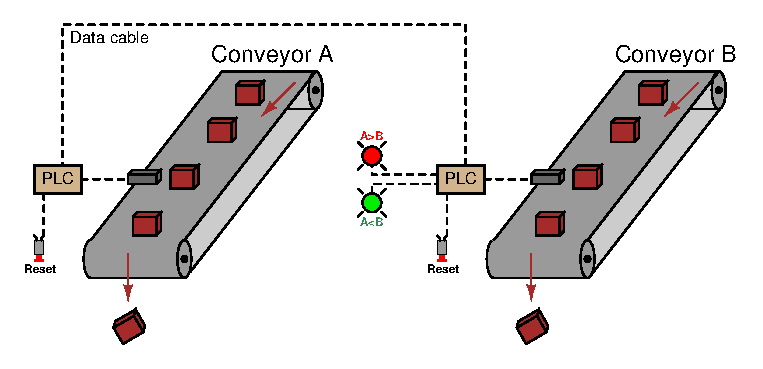
\includegraphics[width=15.5cm]{i02493x01.eps}$$

\vskip 10pt

Work individually or in teams to write a PLC program comparing the two conveyor belts' parts counts using network communication instructions.  Each PLC needs to have its own dedicated ``reset'' switch to reset that conveyor's part counter individually.  {\it Note: some PLC models do not support the network communication ability required in this programming challenge.  The Allen-Bradley MicroLogix 1000 series A and B PLCs fall into this category, being able to only respond to message queries from other PLCs, not initiate their own queries of other PLCs.}

\vskip 10pt

When your system is complete and tested, capture a screen-shot of the PLC program as it appears on your computer, and prepare to present your program solution to the class in a review session for everyone to see and critique.  The purpose of this review session is to see multiple solutions to one problem, explore different programming techniques, and gain experience interpreting PLC programs others have written.  When presenting your program (either individually or as a team), prepare to discuss the following points:

\begin{itemize}
\item{} Show how the communication command(s) is set up, including all the relevant parameters such as baud rate, parity bits, stop bits (which must be set identically in the PLC and the other device).
\item{} Identify which Modbus codes were used to read and/or write information with the other device.
\item{} If multiple communication instructions were used in the PLC program, show how you programmed the PLC so these instructions would not interfere with each other (because they are each using the same communications port on the PLC).
\item{} How you designed the program (i.e. what steps you took to go from a concept to a working program)
\end{itemize}

\vskip 20pt \vbox{\hrule \hbox{\strut \vrule{} {\bf Suggestions for Socratic discussion} \vrule} \hrule}

\begin{itemize}
\item{} Would you recommend one PLC in this system execute two counter functions (one for each conveyor), or would you recommend each PLC does its own counting?  Explain your reasoning!
\item{} If you program your system for duplex communication (i.e. the ``master'' PLC both reading from and writing to the ``slave'' PLC), how do you coordinate the communication instructions so that the ``read'' and ``write'' instructions happen at different times and never simultaneously?
\end{itemize}

\vfil 

\underbar{file i02493}
\eject
%(END_QUESTION)





%(BEGIN_ANSWER)


%(END_ANSWER)





%(BEGIN_NOTES)

As with most PLC systems where process data gets transferred between PLCs, there is more than one way to do it.  Here, we could have one PLC perform both counting functions (passing discrete sensor data over the network from the remote PLC to the one doing the counting for both conveyors) or we could have each PLC do its own counting (passing the remote PLC's count accumulator value over the network for comparison).

Between these two approaches, I would recommend the one where each PLC locally runs its own counter.  This makes it so that if the data network between PLCs ever becomes severed, the remote PLC's counting data is not lost, and the system will pick back up as normal once the severed connection is repaired.

\vskip 10pt

I strongly recommend students save all their PLC programs for future reference, commenting them liberally and saving them with special filenames for easy searching at a later date!

\vskip 10pt

I also recommend presenting these programs as problems for students to work on in class for a short time period, then soliciting screenshot submissions from students (on flash drive, email, or some other electronic file transfer method) when that short time is up.  The purpose of this is to get students involved in PLC programming, and also to have them see other students' solutions to the same problem.  These screenshots may be emailed back to students at the conclusion of the day so they have other students' efforts to reference for further study.


%INDEX% PLC, programming challenge: remote object counting/comparison
%INDEX% Process: conveyor belt item counting

%(END_NOTES)


